
%% bare_conf.tex
%% V1.4b
%% 2015/08/26
%% by Michael Shell
%% See:
%% http://www.michaelshell.org/
%% for current contact information.
%%
%% This is a skeleton file demonstrating the use of IEEEtran.cls
%% (requires IEEEtran.cls version 1.8b or later) with an IEEE
%% conference paper.
%%
%% Support sites:
%% http://www.michaelshell.org/tex/ieeetran/
%% http://www.ctan.org/pkg/ieeetran
%% and
%% http://www.ieee.org/

%%*************************************************************************
%% Legal Notice:
%% This code is offered as-is without any warranty either expressed or
%% implied; without even the implied warranty of MERCHANTABILITY or
%% FITNESS FOR A PARTICULAR PURPOSE! 
%% User assumes all risk.
%% In no event shall the IEEE or any contributor to this code be liable for
%% any damages or losses, including, but not limited to, incidental,
%% consequential, or any other damages, resulting from the use or misuse
%% of any information contained here.
%%
%% All comments are the opinions of their respective authors and are not
%% necessarily endorsed by the IEEE.
%%
%% This work is distributed under the LaTeX Project Public License (LPPL)
%% ( http://www.latex-project.org/ ) version 1.3, and may be freely used,
%% distributed and modified. A copy of the LPPL, version 1.3, is included
%% in the base LaTeX documentation of all distributions of LaTeX released
%% 2003/12/01 or later.
%% Retain all contribution notices and credits.
%% ** Modified files should be clearly indicated as such, including  **
%% ** renaming them and changing author support contact information. **
%%*************************************************************************


% *** Authors should verify (and, if needed, correct) their LaTeX system  ***
% *** with the testflow diagnostic prior to trusting their LaTeX platform ***
% *** with production work. The IEEE's font choices and paper sizes can   ***
% *** trigger bugs that do not appear when using other class files.       ***                          ***
% The testflow support page is at:
% http://www.michaelshell.org/tex/testflow/



\documentclass[conference]{IEEEtran}
% Some Computer Society conferences also require the compsoc mode option,
% but others use the standard conference format.
%
% If IEEEtran.cls has not been installed into the LaTeX system files,
% manually specify the path to it like:
% \documentclass[conference]{../sty/IEEEtran}





% Some very useful LaTeX packages include:
% (uncomment the ones you want to load)


% *** MISC UTILITY PACKAGES ***
%
%\usepackage{ifpdf}
% Heiko Oberdiek's ifpdf.sty is very useful if you need conditional
% compilation based on whether the output is pdf or dvi.
% usage:
% \ifpdf
%   % pdf code
% \else
%   % dvi code
% \fi
% The latest version of ifpdf.sty can be obtained from:
% http://www.ctan.org/pkg/ifpdf
% Also, note that IEEEtran.cls V1.7 and later provides a builtin
% \ifCLASSINFOpdf conditional that works the same way.
% When switching from latex to pdflatex and vice-versa, the compiler may
% have to be run twice to clear warning/error messages.






% *** CITATION PACKAGES ***
%
%\usepackage{cite}
% cite.sty was written by Donald Arseneau
% V1.6 and later of IEEEtran pre-defines the format of the cite.sty package
% \cite{} output to follow that of the IEEE. Loading the cite package will
% result in citation numbers being automatically sorted and properly
% "compressed/ranged". e.g., [1], [9], [2], [7], [5], [6] without using
% cite.sty will become [1], [2], [5]--[7], [9] using cite.sty. cite.sty's
% \cite will automatically add leading space, if needed. Use cite.sty's
% noadjust option (cite.sty V3.8 and later) if you want to turn this off
% such as if a citation ever needs to be enclosed in parenthesis.
% cite.sty is already installed on most LaTeX systems. Be sure and use
% version 5.0 (2009-03-20) and later if using hyperref.sty.
% The latest version can be obtained at:
% http://www.ctan.org/pkg/cite
% The documentation is contained in the cite.sty file itself.





\usepackage{url}
\usepackage[fleqn]{amsmath}
\usepackage{algorithm,algpseudocode}
\usepackage{mathtools}


% *** GRAPHICS RELATED PACKAGES ***
%
\ifCLASSINFOpdf
  % \usepackage[pdftex]{graphicx}
  % declare the path(s) where your graphic files are
  % \graphicspath{{../pdf/}{../jpeg/}}
  % and their extensions so you won't have to specify these with
  % every instance of \includegraphics
  % \DeclareGraphicsExtensions{.pdf,.jpeg,.png}
\else
  % or other class option (dvipsone, dvipdf, if not using dvips). graphicx
  % will default to the driver specified in the system graphics.cfg if no
  % driver is specified.
  % \usepackage[dvips]{graphicx}
  % declare the path(s) where your graphic files are
  % \graphicspath{{../eps/}}
  % and their extensions so you won't have to specify these with
  % every instance of \includegraphics
  % \DeclareGraphicsExtensions{.eps}
\fi
% graphicx was written by David Carlisle and Sebastian Rahtz. It is
% required if you want graphics, photos, etc. graphicx.sty is already
% installed on most LaTeX systems. The latest version and documentation
% can be obtained at: 
% http://www.ctan.org/pkg/graphicx
% Another good source of documentation is "Using Imported Graphics in
% LaTeX2e" by Keith Reckdahl which can be found at:
% http://www.ctan.org/pkg/epslatex
%
% latex, and pdflatex in dvi mode, support graphics in encapsulated
% postscript (.eps) format. pdflatex in pdf mode supports graphics
% in .pdf, .jpeg, .png and .mps (metapost) formats. Users should ensure
% that all non-photo figures use a vector format (.eps, .pdf, .mps) and
% not a bitmapped formats (.jpeg, .png). The IEEE frowns on bitmapped formats
% which can result in "jaggedy"/blurry rendering of lines and letters as
% well as large increases in file sizes.
%
% You can find documentation about the pdfTeX application at:
% http://www.tug.org/applications/pdftex





% *** MATH PACKAGES ***
%
%\usepackage{amsmath}
% A popular package from the American Mathematical Society that provides
% many useful and powerful commands for dealing with mathematics.
%
% Note that the amsmath package sets \interdisplaylinepenalty to 10000
% thus preventing page breaks from occurring within multiline equations. Use:
%\interdisplaylinepenalty=2500
% after loading amsmath to restore such page breaks as IEEEtran.cls normally
% does. amsmath.sty is already installed on most LaTeX systems. The latest
% version and documentation can be obtained at:
% http://www.ctan.org/pkg/amsmath





% *** SPECIALIZED LIST PACKAGES ***
%
%\usepackage{algorithmic}
% algorithmic.sty was written by Peter Williams and Rogerio Brito.
% This package provides an algorithmic environment fo describing algorithms.
% You can use the algorithmic environment in-text or within a figure
% environment to provide for a floating algorithm. Do NOT use the algorithm
% floating environment provided by algorithm.sty (by the same authors) or
% algorithm2e.sty (by Christophe Fiorio) as the IEEE does not use dedicated
% algorithm float types and packages that provide these will not provide
% correct IEEE style captions. The latest version and documentation of
% algorithmic.sty can be obtained at:
% http://www.ctan.org/pkg/algorithms
% Also of interest may be the (relatively newer and more customizable)
% algorithmicx.sty package by Szasz Janos:
% http://www.ctan.org/pkg/algorithmicx




% *** ALIGNMENT PACKAGES ***
%
%\usepackage{array}
% Frank Mittelbach's and David Carlisle's array.sty patches and improves
% the standard LaTeX2e array and tabular environments to provide better
% appearance and additional user controls. As the default LaTeX2e table
% generation code is lacking to the point of almost being broken with
% respect to the quality of the end results, all users are strongly
% advised to use an enhanced (at the very least that provided by array.sty)
% set of table tools. array.sty is already installed on most systems. The
% latest version and documentation can be obtained at:
% http://www.ctan.org/pkg/array


% IEEEtran contains the IEEEeqnarray family of commands that can be used to
% generate multiline equations as well as matrices, tables, etc., of high
% quality.




% *** SUBFIGURE PACKAGES ***
%\ifCLASSOPTIONcompsoc
%  \usepackage[caption=false,font=normalsize,labelfont=sf,textfont=sf]{subfig}
%\else
%  \usepackage[caption=false,font=footnotesize]{subfig}
%\fi
% subfig.sty, written by Steven Douglas Cochran, is the modern replacement
% for subfigure.sty, the latter of which is no longer maintained and is
% incompatible with some LaTeX packages including fixltx2e. However,
% subfig.sty requires and automatically loads Axel Sommerfeldt's caption.sty
% which will override IEEEtran.cls' handling of captions and this will result
% in non-IEEE style figure/table captions. To prevent this problem, be sure
% and invoke subfig.sty's "caption=false" package option (available since
% subfig.sty version 1.3, 2005/06/28) as this is will preserve IEEEtran.cls
% handling of captions.
% Note that the Computer Society format requires a larger sans serif font
% than the serif footnote size font used in traditional IEEE formatting
% and thus the need to invoke different subfig.sty package options depending
% on whether compsoc mode has been enabled.
%
% The latest version and documentation of subfig.sty can be obtained at:
% http://www.ctan.org/pkg/subfig




% *** FLOAT PACKAGES ***
%
%\usepackage{fixltx2e}
% fixltx2e, the successor to the earlier fix2col.sty, was written by
% Frank Mittelbach and David Carlisle. This package corrects a few problems
% in the LaTeX2e kernel, the most notable of which is that in current
% LaTeX2e releases, the ordering of single and double column floats is not
% guaranteed to be preserved. Thus, an unpatched LaTeX2e can allow a
% single column figure to be placed prior to an earlier double column
% figure.
% Be aware that LaTeX2e kernels dated 2015 and later have fixltx2e.sty's
% corrections already built into the system in which case a warning will
% be issued if an attempt is made to load fixltx2e.sty as it is no longer
% needed.
% The latest version and documentation can be found at:
% http://www.ctan.org/pkg/fixltx2e


%\usepackage{stfloats}
% stfloats.sty was written by Sigitas Tolusis. This package gives LaTeX2e
% the ability to do double column floats at the bottom of the page as well
% as the top. (e.g., "\begin{figure*}[!b]" is not normally possible in
% LaTeX2e). It also provides a command:
%\fnbelowfloat
% to enable the placement of footnotes below bottom floats (the standard
% LaTeX2e kernel puts them above bottom floats). This is an invasive package
% which rewrites many portions of the LaTeX2e float routines. It may not work
% with other packages that modify the LaTeX2e float routines. The latest
% version and documentation can be obtained at:
% http://www.ctan.org/pkg/stfloats
% Do not use the stfloats baselinefloat ability as the IEEE does not allow
% \baselineskip to stretch. Authors submitting work to the IEEE should note
% that the IEEE rarely uses double column equations and that authors should try
% to avoid such use. Do not be tempted to use the cuted.sty or midfloat.sty
% packages (also by Sigitas Tolusis) as the IEEE does not format its papers in
% such ways.
% Do not attempt to use stfloats with fixltx2e as they are incompatible.
% Instead, use Morten Hogholm'a dblfloatfix which combines the features
% of both fixltx2e and stfloats:
%
% \usepackage{dblfloatfix}
% The latest version can be found at:
% http://www.ctan.org/pkg/dblfloatfix




% *** PDF, URL AND HYPERLINK PACKAGES ***
%
%\usepackage{url}
% url.sty was written by Donald Arseneau. It provides better support for
% handling and breaking URLs. url.sty is already installed on most LaTeX
% systems. The latest version and documentation can be obtained at:
% http://www.ctan.org/pkg/url
% Basically, \url{my_url_here}.




% *** Do not adjust lengths that control margins, column widths, etc. ***
% *** Do not use packages that alter fonts (such as pslatex).         ***
% There should be no need to do such things with IEEEtran.cls V1.6 and later.
% (Unless specifically asked to do so by the journal or conference you plan
% to submit to, of course. )


% correct bad hyphenation here
\hyphenation{op-tical net-works semi-conduc-tor}


\begin{document}
%
% paper title
% Titles are generally capitalized except for words such as a, an, and, as,
% at, but, by, for, in, nor, of, on, or, the, to and up, which are usually
% not capitalized unless they are the first or last word of the title.
% Linebreaks \\ can be used within to get better formatting as desired.
% Do not put math or special symbols in the title.
\title{Raspberry Pi GoPiGo Robot\\EKF SLAM Implementation}


% author names and affiliations
% use a multiple column layout for up to three different
% affiliations
\author{\IEEEauthorblockN{Gopal Menon}
\IEEEauthorblockA{Computer Science Department\\
Utah State University\\
Logan, Utah 84322\\
Email: gopal.menon@aggiemail.usu.edu}
}

% conference papers do not typically use \thanks and this command
% is locked out in conference mode. If really needed, such as for
% the acknowledgment of grants, issue a \IEEEoverridecommandlockouts
% after \documentclass

% for over three affiliations, or if they all won't fit within the width
% of the page, use this alternative format:
% 
%\author{\IEEEauthorblockN{Michael Shell\IEEEauthorrefmark{1},
%Homer Simpson\IEEEauthorrefmark{2},
%James Kirk\IEEEauthorrefmark{3}, 
%Montgomery Scott\IEEEauthorrefmark{3} and
%Eldon Tyrell\IEEEauthorrefmark{4}}
%\IEEEauthorblockA{\IEEEauthorrefmark{1}School of Electrical and Computer Engineering\\
%Georgia Institute of Technology,
%Atlanta, Georgia 30332--0250\\ Email: see http://www.michaelshell.org/contact.html}
%\IEEEauthorblockA{\IEEEauthorrefmark{2}Twentieth Century Fox, Springfield, USA\\
%Email: homer@thesimpsons.com}
%\IEEEauthorblockA{\IEEEauthorrefmark{3}Starfleet Academy, San Francisco, California 96678-2391\\
%Telephone: (800) 555--1212, Fax: (888) 555--1212}
%\IEEEauthorblockA{\IEEEauthorrefmark{4}Tyrell Inc., 123 Replicant Street, Los Angeles, California 90210--4321}}




% use for special paper notices
%\IEEEspecialpapernotice{(Invited Paper)}




% make the title area
\maketitle

% As a general rule, do not put math, special symbols or citations
% in the abstract
\begin{abstract}
Robot motion is stochastic and not deterministic. A robot does not faithfully execute movement commands due to inaccuracies in its motion mechanism, approximations made in modelling its environment and incomplete modelling of the physics of its operating environment. Due to these reasons, the robot may not end up exactly at the location where it should have been if the movement command had been faithfully executed. The robot position may be thought of as a two dimensional probability distribution. This probability distribution will have a mean that will be equal to the expected robot location based on the movement command. The covariance will be the measure of how faithfully it executes commands. Due to this uncertainty in movement, with each motion command, the location uncertainty increases and after a while the robot gets lost. In some applications, robots need to be able to go into an unknown environment and explore it. This is a difficult problem due to the issue described above. If a map of the environment is available, the robot can use sensors to find its location in the environment. Conversely, if the robot knows where it is, it can generate an environment map. This is a sort of chicken and end problem. Simultaneous Localization and Mapping (SLAM) solves this problem. An Extended Kalman Filter (EKF) can be used to reduce robot location uncertainty. This is done by combining the predicted robot location based on the equation of robot motion with the measured location based on sensor readings. The two robot location estimates are Gaussian distributions. These two distributions are combined and the resulting distribution will have a mean that is closer to the location estimate with the lower uncertainty and the uncertainty of resulting location will be lower than either of the two distributions (see \ref{sssec:num1}). This document describes the implementation of EKF SLAM using a robot.
\end{abstract}

% no keywords




% For peer review papers, you can put extra information on the cover
% page as needed:
% \ifCLASSOPTIONpeerreview
% \begin{center} \bfseries EDICS Category: 3-BBND \end{center}
% \fi
%
% For peerreview papers, this IEEEtran command inserts a page break and
% creates the second title. It will be ignored for other modes.
\IEEEpeerreviewmaketitle

\section{Introduction}
% no \IEEEPARstart
\subsection{The robot platform}
The robot used for this implementation is based on a Raspberry Pi and is manufactured and sold by Dexter Industries \cite{dexter}. The robot is equipped with an ultrasonic sensor that is capable of measuring distances accurately to 250 cm. The sensor is mounted on a servo mechanism that can point the sensor in any direction ahead of the robot. The robot moves through use of two wheels that can be independently controlled by motors. Each wheel has an encoder using which the robot can issue commands for a wheel to move a fixed number of steps. The robot also has a third castor wheel that can move in any direction, but is not powered. The robot will be given commands to make it move and it can sense its surroundings using the ultrasonic sensor.
\subsection{EKF SLAM}
A Kalman filter is a Gaussian filter algorithm that can use two Gaussian distributions for a computed value and merge them together to form a distribution that has lesser variance than either of the two distributions. A Kalman filter however only works in the case of systems where the mechanics are linear. This is where the Extended Kalman Filter (EKF) comes in. An EKF uses an approximation to find the resultant distribution after a prior distribution is transformed by a non-linear function. The robot movement and landmark sensing is governed by trigonometric functions that are based on the angle of the robot orientation. These functions are non-linear since they are trigonometric.\\

The robot will compute its expected position based on its prior position and the movement command. This is the prediction step. It will also make independent estimates of its position using the bearing and range to known landmarks returned by its ultrasonic sensor. These two measurements will be combined through use of an EKF in such a way that the position uncertainty is reduced. The Kalman Gain or the reduction in the robot position uncertainty is inversely proportional to the sensor uncertainty. The better the sensor, the higher will be the Kalman Gain and the less uncertainty there will be in the robot position\cite{stachniss}.

\section{Problem Statement}
\subsection{Location Uncertainty}

\begin{figure}[!t]
\centering
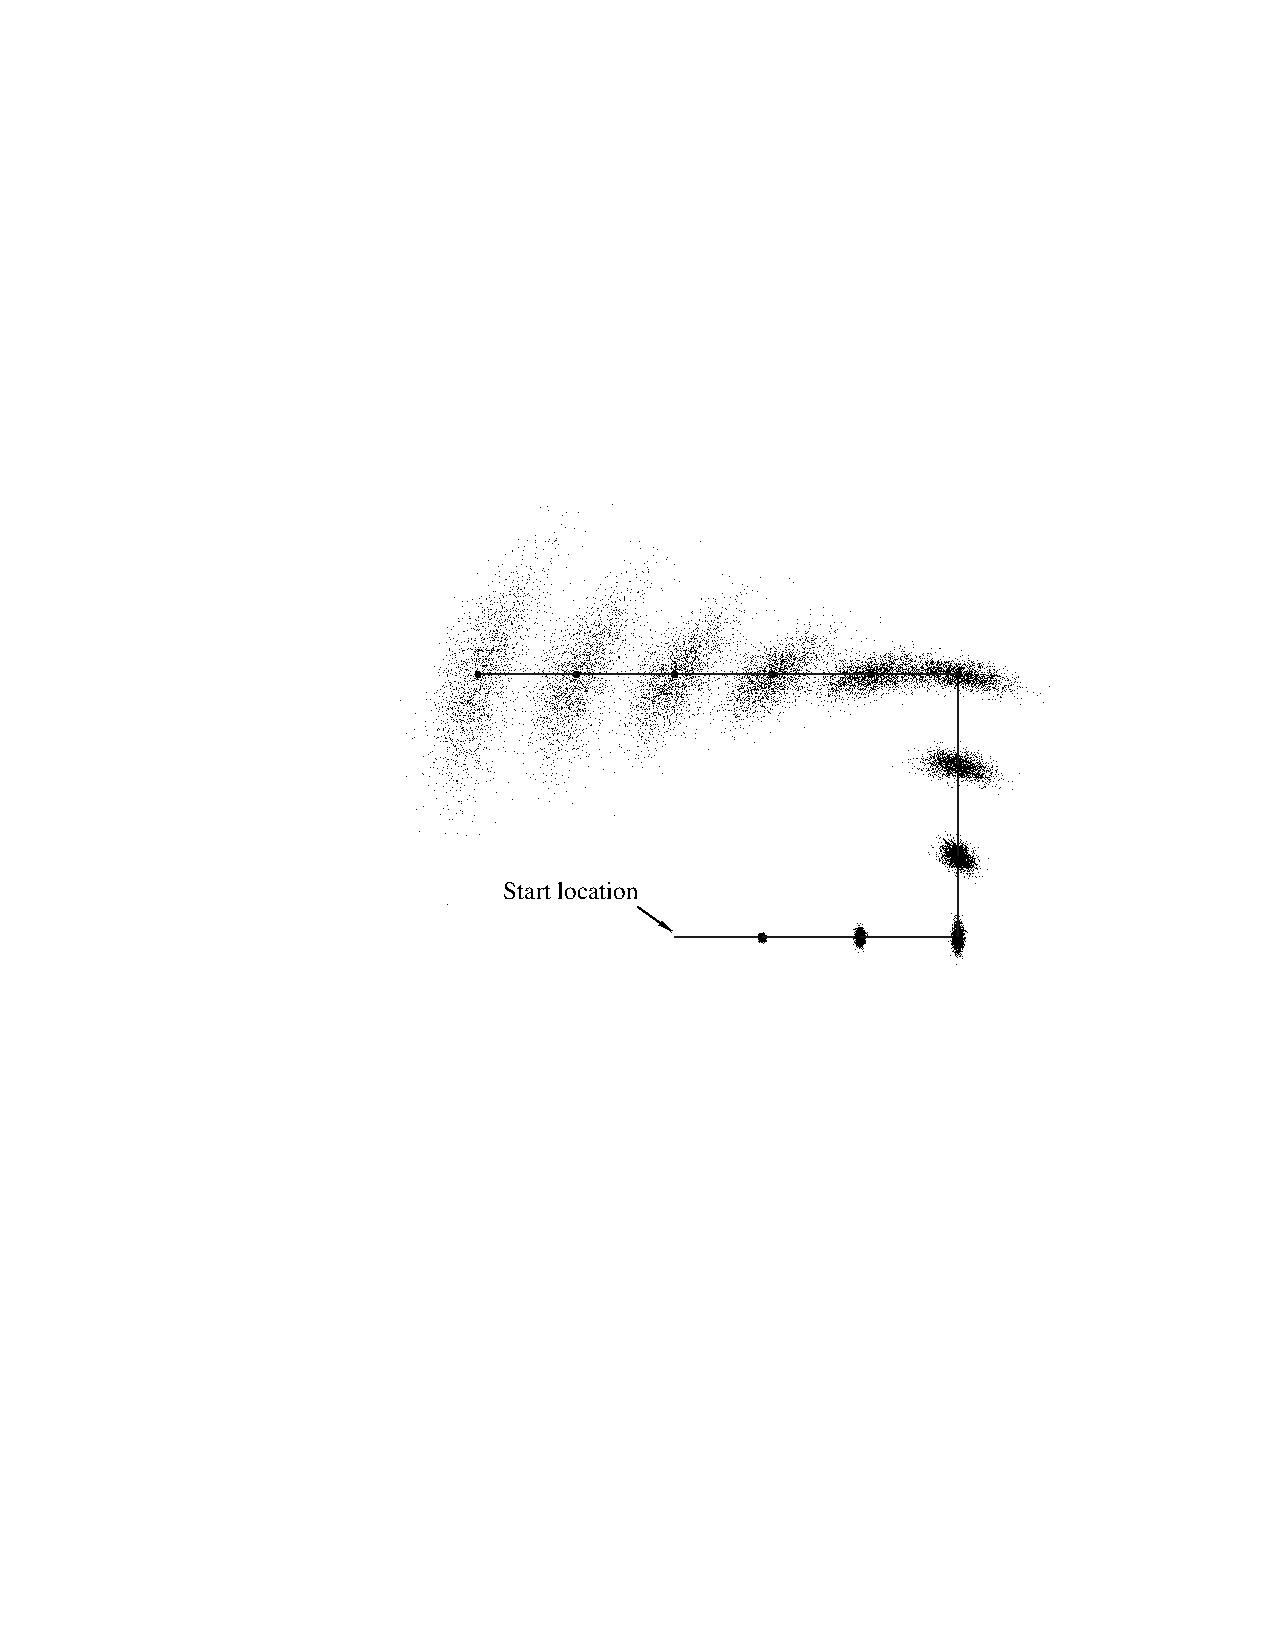
\includegraphics[width=3.5in]{./figures/LostRobot.pdf}
\caption{Sampling approximation of the position belief for a non-sensing robot \cite{thrun}. The solid line displays the actions, and the samples represent the robot’s belief at different points in time.}
\label{LostRobot}
\end{figure}

As described above, robot motion is stochastic and not deterministic. Due to  uncertainty in movement, with each motion command, the location uncertainty increases and after a while the robot gets lost.\\

Figure \ref{LostRobot} shows the location uncertainty problem. Before the robot starts moving, it knows exactly where it is. So it's location belief is a single point. After each movement, its location uncertainty increases. This is shown by the location probability distribution that changes from a point to a larger area with the first step and the uncertainty, shown by an ellipse shaped point distribution,  increasing in size with each step. In the final position of the robot, the uncertainty is the largest as it accumulates the added uncertainty with each step.\\

This increasing uncertainty is a problem that eventually results in a lost robot that does not know where it is.

\section{Approach/Methods}

The following sections provide some background material that is required for understanding the solution to the robot localization problem.

\subsection{The Bayes Filter}

The Bayes Filter is an algorithm used for calculating beliefs \cite{thrun}. In our case it is the belief of the robot position. This algorithm is used to compute the belief probability distribution $bel$ from measurement and control data. The measurement data is obtained from sensors and the control data is obtained from the robot motion command or telemetry readings.\\

The robot will keep track of its current location as it moves. When it issues a movement command, it can compute its expected location after the move command is executed. This is the control data. It can use its sensors and obtain the range and bearing to known landmarks. Using this, it can compute its expected location. This is the measurement data.\\

Bayes Rule says that

\begin{equation}\label{BayesRule}
p(x|y) = \frac{p(y|x) p(x)}{p(y)}
\end{equation}

Since the denominator in Bayes Rule does not depend on $x$, the factor $\frac{1}{p(y)}$ can be written as $\eta$. So Bayes Rule in equation \ref{BayesRule} can be written as

\begin{equation}\label{BayesRuleEta}
p(x|y) = \eta p(y|x) p(x)
\end{equation}

Bayes Rule \ref{BayesRule} can also be written as 

\begin{equation}\label{BayesRuleCondZ}
p(x|y,z) = \frac{p(y|x,z) p(x|z)}{p(y|z)}
\end{equation}

as long as $p(y|z)>0$.\\

Applying \ref{BayesRuleCondZ} on the robot position $x_t$ at time $t$ for measurements $z_{1:t}$ and commands $u_{1:t}$ gi	-ves us

\begin{equation}\label{TargetPosterior}
\begin{aligned}
p(x_t|z_{1:t},u_{1:t}) &= \frac{p(z_t|x_t,z_{1:t-1},u_{1:t}) p(x_t|z_{1:t-1},u_{1:t})}{p(z_t|z_{1:t-1},u_{1:t})}\\
& = \eta p(z_t|x_t,z_{1:t-1},u_{1:t}) p(x_t|z_{1:t-1},u_{1:t})\\
\end{aligned}
\end{equation}

Since the measurement $z_t$ depends on position $x_t$ and any past measurement $z_{1:t}$ or command $u_{1:t} $ does not provide any additional information on the measurement, we can say that

\begin{equation}\label{SimplTargPost}
p(z_t|x_t,z_{1:t-1},u_{1:t}) = p(z_t|x_t)
\end{equation}

This allows us to simplify \ref{TargetPosterior} as

\begin{equation}\label{MoreSimplTargPost}
\begin{aligned}
p(x_t|z_{1:t},u_{1:t}) &= \eta p(z_t|x_t) p(x_t|z_{1:t-1}, u_{1:t})\\
&= \eta p(z_t|x_t) \overline{bel}(x_t)
\end{aligned}
\end{equation}

where

\begin{equation}\label{belief}
\overline{bel}(x_t) = p(x_t|z_{1:t-1}, u_{1:t})
\end{equation}

Using the theorem of total probability

\begin{equation}
p(x) = \int p(x|y) p(y) dy
\end{equation}

equation \ref{belief} can be written as 

\begin{equation}
\overline{bel}(x_t) = \int p(x_t|x_{t-1}, z_{1:t-1}, u_{1:t}) p(x_{t-1}|z_{1:t-1}, u_{1:t}) dx_{t-1}
\end{equation}

If we know the state $x_{t-1}$, past measurements and controls have no bearing on the state $x_t$. So

\begin{equation}
p(x_t|x_{t-1}, z_{1:t-1}, u_{1:t}) = p(x_t|x_{t-1}, u_t)
\end{equation}

We can see that command $u_t$ can be omitted from the set of conditioning variables in $p(x_{t-1}|z_{1:t-1}, u_{1:t})$. This gives us the recursive update equation \ref{belief} as

\begin{equation}
\overline{bel}(x_t) = \int p(x_t|x_{t-1}, u_t) p(x_{t-1}|z_{1:t-1}, u_{1:t-1}) dx_{t-1}
\end{equation}

This reduces to

\begin{equation}
\overline{bel}(x_t) = \int p(x_t|x_{t-1}, u_t) bel(x_{t-1}) dx_{t-1}
\end{equation}

\subsection{The Bayes Filter Algorithm}

Based on the above mathematical derivation for a Bayes Filter, we can write down the Bayes Filter Algorithm as follows \cite{thrun}

\begin{minipage}{\linewidth}
  \begin{algorithm}[H]
    \caption{Bayes Filter Algorithm}\label{AlgBayes}
    \begin{algorithmic}[1]
      \Procedure{BayesFilterAlgorithm}{$bel(x_{t-1},u_t, z_t)$}
	\For{all $x_t$}
		\State $\overline{bel}(x_t) = \int p(x_t|x_{t-1}, u_t) bel(x_{t-1}) dx_{t-1}$
		\State $bel(x_t)= \eta p(z_t|x_t) \overline{bel}(x_t)$
	\EndFor
      \EndProcedure
    \end{algorithmic}
  \end{algorithm}
\end{minipage}\\\\

The belief $bel(x_t)$ at time $t$ is computed from the belief $bel(x_{t-1})$ at time $t-1$. The input to the algorithm is the belief $bel$ at time $t-1$, along with the most recent control value $u_t$ and the most recent measurement $z_t$. Its output is the belief $bel(x_t)$ at time $t$.\\

The Bayes Filter Algorithm consist of two essentials steps. In line 3, which is the prediction step, it calculates its belief over state $x_t$ based on the prior belief over state $x_{t-1}$ and the control $u_t$. The belief $\overline{bel}(x_t)$ that the robot assigns to state $x_t$ is obtained by the integral (or in other words the sum) of the product of two distributions: the prior assigned to $x_{t-1}$, and the probability that control $u_t$ induces a transition from $x_{t-1}$ to $x_t$.\\

The second step of the Bayes Filter is called the measurement update. In line 4, the Bayes Filter algorithm multiplies the belief $\overline{bel}(x_t)$ by the probability that the measurement $z_t$ may have been observed. It does this for every hypothetical posterior state $x_t$.

\subsection{The Kalman Filter}

The Kalman Filter is a technique for implementing a Bayes Filter  \cite{thrun}. This is used for filtering and prediction in linear Gaussian systems.\\

A probability distribution of a one-dimensional normal distribution with mean $\mu$ and variance $\sigma ^2$ is given by the following Gaussian function
 
 \begin{equation}\label{1dNormal}
p(x) = (2 \pi \sigma ^ 2) ^ {-\frac{1}{2}} \exp\left\{ - \frac{1}{2} \frac{(x - \mu)^2}{\sigma ^ 2} \right\}
\end{equation}

The Normal distribution \ref{1dNormal} is for a scalar $x$. In the case of a robot, the robot location on a flat surface is given by $\begin{bmatrix} x &   y & \theta \end{bmatrix}^{T}$ where $x$ is the x coordinate, $y$ is the y coordinate and $\theta$ is the robot orientation. This vector is called the robot pose. A Normal distribution over such a vector is called \textit{multivariate}. These distributions have the following form

 \begin{equation}\label{MvNormal}
p(x) = \det(2 \pi \Sigma) ^ {-\frac{1}{2}} \exp\left\{ - \frac{1}{2} (x - \mu)^T \Sigma ^ {-1} (x - \mu) \right\}
\end{equation}

where $\mu$ is the mean vector that has the same dimensionality as the state $x$. $\Sigma$ is the covariance matrix and its dimension is the dimensionality of the state $x$ squared. Equation \ref{MvNormal} is a generalization of equation \ref{1dNormal}. Both definitions are equivalent if $x$ is a scalar and value and $\Sigma = \sigma ^ 2$.

For a Kalman filter, in posteriors are Gaussian if the following three properties hold\\

\begin{enumerate}
\item The state transition probability $p(x_t|x_{t-1}, u_t)$ must be a linear function of its arguments with added Gaussian noise. This is expressed by the following equation

 \begin{equation}\label{Kalman1}
x_t = A_tx_{t-1} + B_tu_t + \varepsilon_t
\end{equation}

where $A_t$ and $B_t$ are matrices. $A_t$ has the dimension equal to the square of the state vector, $B_t$ has the dimension of $n \times m$, where $n$ is the dimension of the state vector and $m$ is the dimension of the control variable $u_t$. The random variable $\varepsilon_t$ models the uncertainty introduced by the state transition and depends on the robot mechanics. Its mean is zero and covariance will be denoted by $R_t$. The state transition probability distribution can be obtained by plugging in \ref{Kalman1} into \ref{MvNormal}. The mean of the posterior state is given by $A_tx_{t-1} + B_tu_t$ and the covariance by $R_t$.\\

\item The measurement probability $p(z_t|x_t)$ must also be linear in its arguments with added Gaussian noise

 \begin{equation}\label{Kalman2}
z_t = C_tx_{t} + \delta_t
\end{equation}

Here $C_t$ is a matrix of size $k \times n$, where $k$ is the dimension of the measurement vector $z_t$. The vector $\delta_t$ describes the measurement noise. The distribution of $\delta_t$ is a multivariate Gaussian with zero mean and covariance $Q_t$.\\

\item Finally the initial belief $bel(x_0)$ must be normally distributed. We can denote the mean of this belief by mean $\mu_0$ and covariance $\Sigma_0$.\\
\end{enumerate}

The Kalman filter algorithm is given below

\begin{minipage}{\linewidth}
  \begin{algorithm}[H]
    \caption{Kalman Filter Algorithm}\label{AlgKalman}
    \begin{algorithmic}[1]
      \Procedure{Kalman Filter Algorithm} {$\mu_{t-1},\Sigma_{t-1}, u_t,z_t$}
	\State $\overline \mu_t = A_t \mu_{t-1} + B_t u_t$
	\State $\overline \Sigma_t= A_t \Sigma_{t-1} A_t^T + R_t$  
	\State $K_t = \overline \Sigma_t C_t^T{(C_t \overline \Sigma_t C_t^T + Q_t)}^{-1}$
	\State $\mu_t = \overline \mu_t + K_t(z_t - C_t \overline \mu_t)$
	\State $\Sigma_t = (I - K_t C_t) \overline \Sigma_t$
	\State return $\mu_t, \Sigma_t$
      \EndProcedure
    \end{algorithmic}
  \end{algorithm}
\end{minipage}\\\\

The algorithm represents the belief $bel(x_t)$ at time $t$ by the mean $\mu_t$ and covariance $\Sigma_t$. The input is the belief at time $t-1$, the covariance at time $t-1$, the control $u_t$ and measurement $z_t$. The output is the belief at time $t$.\\

In lines 2 and 3, the predicted belief $\overline \mu$ and $\overline \Sigma$ is calculated representing the belief $\overline{bel}(x_t)$ one time step later, but before incorporating the measurement $z_t$. This belief is obtained by incorporating the control $u_t$. The mean is updated using the deterministic state transition function \ref{Kalman1} with the mean $\mu_{t-1}$ substituted for the state $x_{t-1}$. The update of the covariance considers the fact that states depend on the previous state through the linear matrix $A_t$. The variable $K_t$ computed in line 4 is called \textit{Kalman gain}. This is the reduction is uncertainty that is obtained by combining the prediction and correction steps. The belief $\overline{bel}(x_t)$ is transformed into the corrected belief ${bel}(x_t)$ in lines 5 and 6 by incorporating the measurement $z_t$. Line 5 manipulates the mean by adjusting it in proportion to the Kalman gain $K_t$ and the deviation of the actual measurement $z_t$ and the measurement predicted as per the measurement probability \ref{Kalman2}. Finally a new covariance of the posterior belief is calculated in line 6, adjusting for the information gain resulting from the measurement.\\

\begin{figure}[!t]
\centering
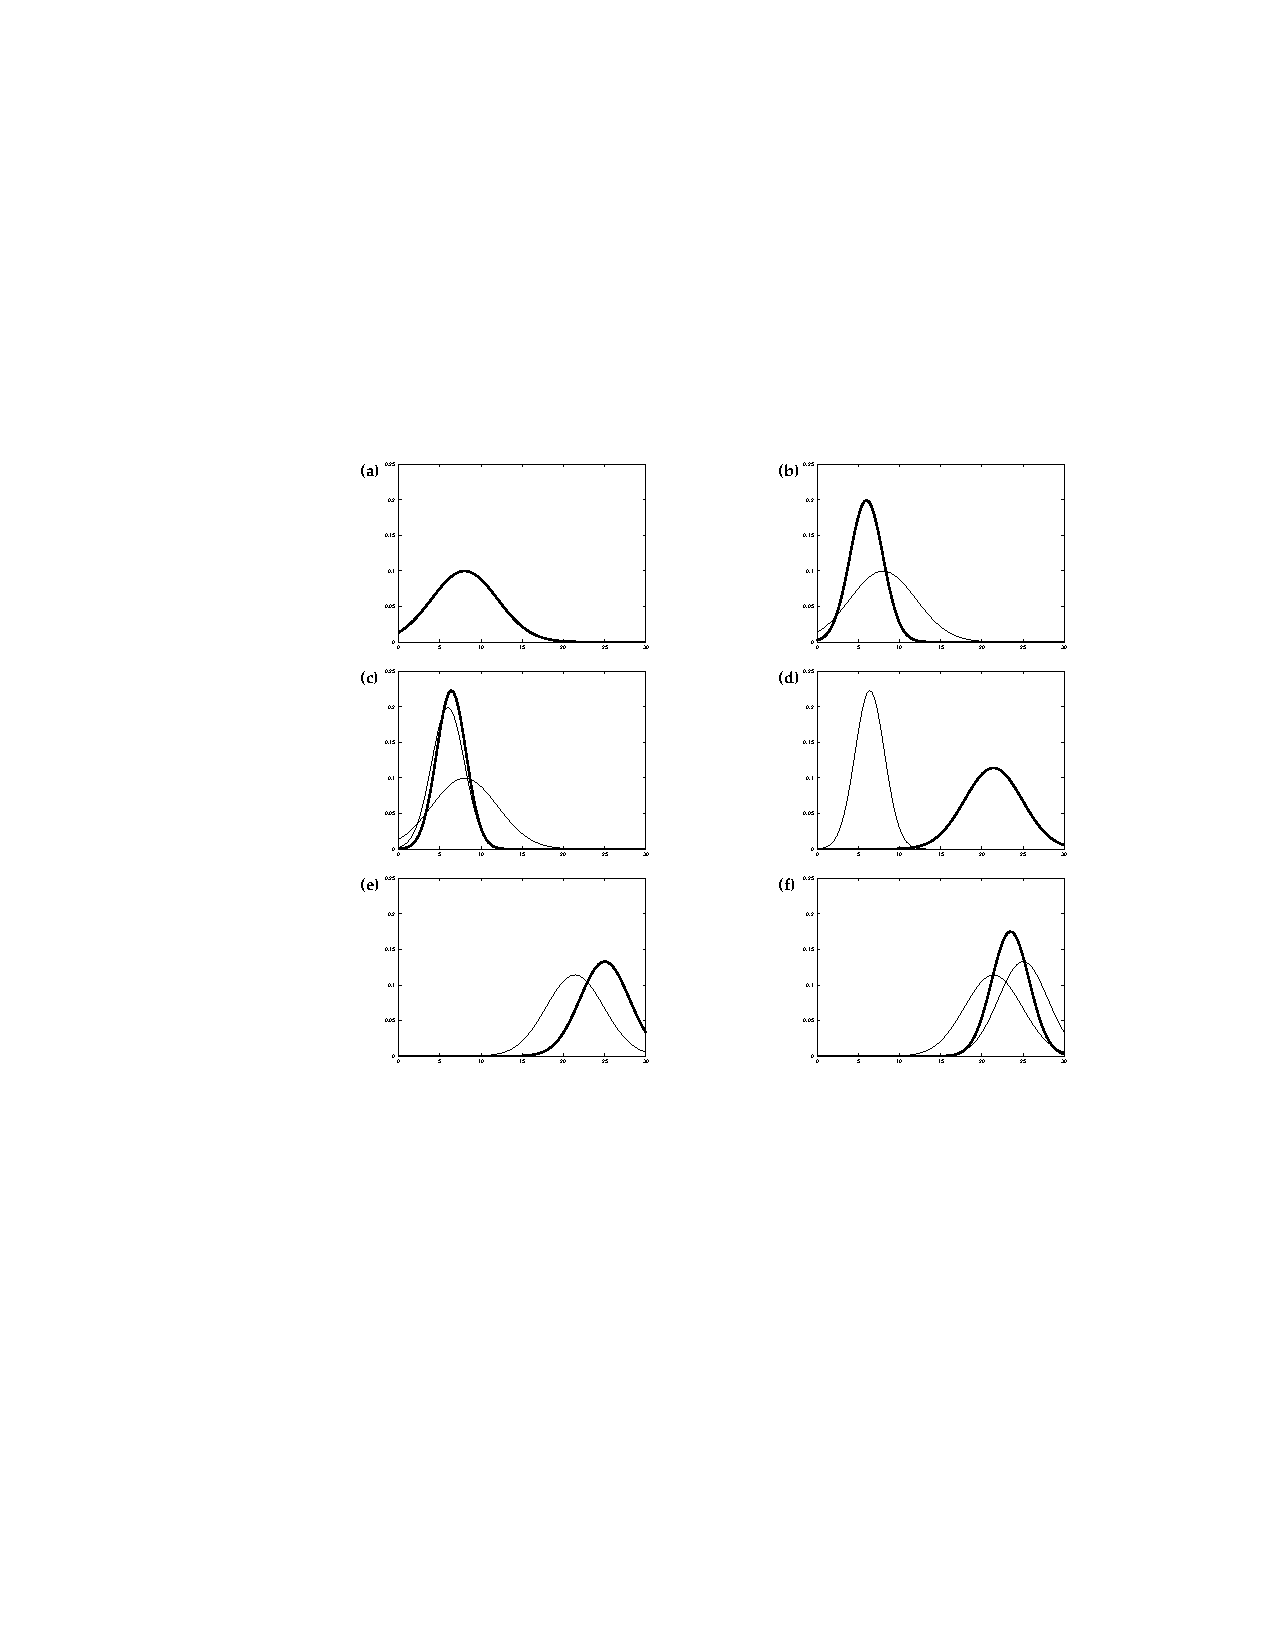
\includegraphics[width=3.5in]{./figures/KalmanIllustration.pdf}

\caption{Illustration of Kalman filters \cite{thrun} (x-axis=location, y-axis=probability of being in that location): (a) initial belief, (b) a measurement (in bold) with the associated uncertainty, (c) belief after integrating the measurement into the belief using the Kalman filter algorithm, (d) belief after motion to the right (which introduces uncertainty), (e) a new measurement with associated uncertainty, and (f) the resulting belief.}
\label{KalmanIllustration}
\end{figure}

Figure \ref{KalmanIllustration} illustrates the Kalman filter for a simplistic one-dimensional localization scenario. Suppose the robot moves in the horizontal axis in each diagram in figure \ref{KalmanIllustration} with the prior over the robot localization given by the normal distribution shown in figure \ref{KalmanIllustration}a. The robot queries its sensors on its location and these return a measurement that is centered at the peak of the bold Gaussian distribution in figure \ref{KalmanIllustration}b. The peak corresponds to the value returned by the sensors and the its width or variance corresponds to the uncertainty in measurement. Combining the prior with the measurement in lines 4 through 6 of the Kalman filter algorithm, yields the bold Gaussian in figure \ref{KalmanIllustration}c. The belief's mean lies between the two original means, and its uncertainty width is smaller than both contributing Gaussians. The is the result of the information gain from using the Kalman filter.\\

Now lets assume that the robot moves towards the right. Its uncertainty grows due to the fact that the state transition is stochastic. Lines 2 and 3 of the Kalman filter algorithm provide us with the Gaussian shown in bold in figure \ref{KalmanIllustration}d. This Gaussian is shifted by the amount the robot moved and is also wider because of the uncertainty introduced by the movement. The robot does a second sensor measurement shown by the bold Gaussian in figure \ref{KalmanIllustration}e, which leads to the posterior shown in bold in figure \ref{KalmanIllustration}f.\\

As this example illustrates, the Kalman filter alternates a measurement update step, in which sensor data is integrated into the present belief, with a prediction step, which modifies the belief. The prediction step increases and the update step decreases the uncertainty in the robot's belief.

\subsection{The Extended Kalman Filter}

\begin{figure}[!t]
\centering
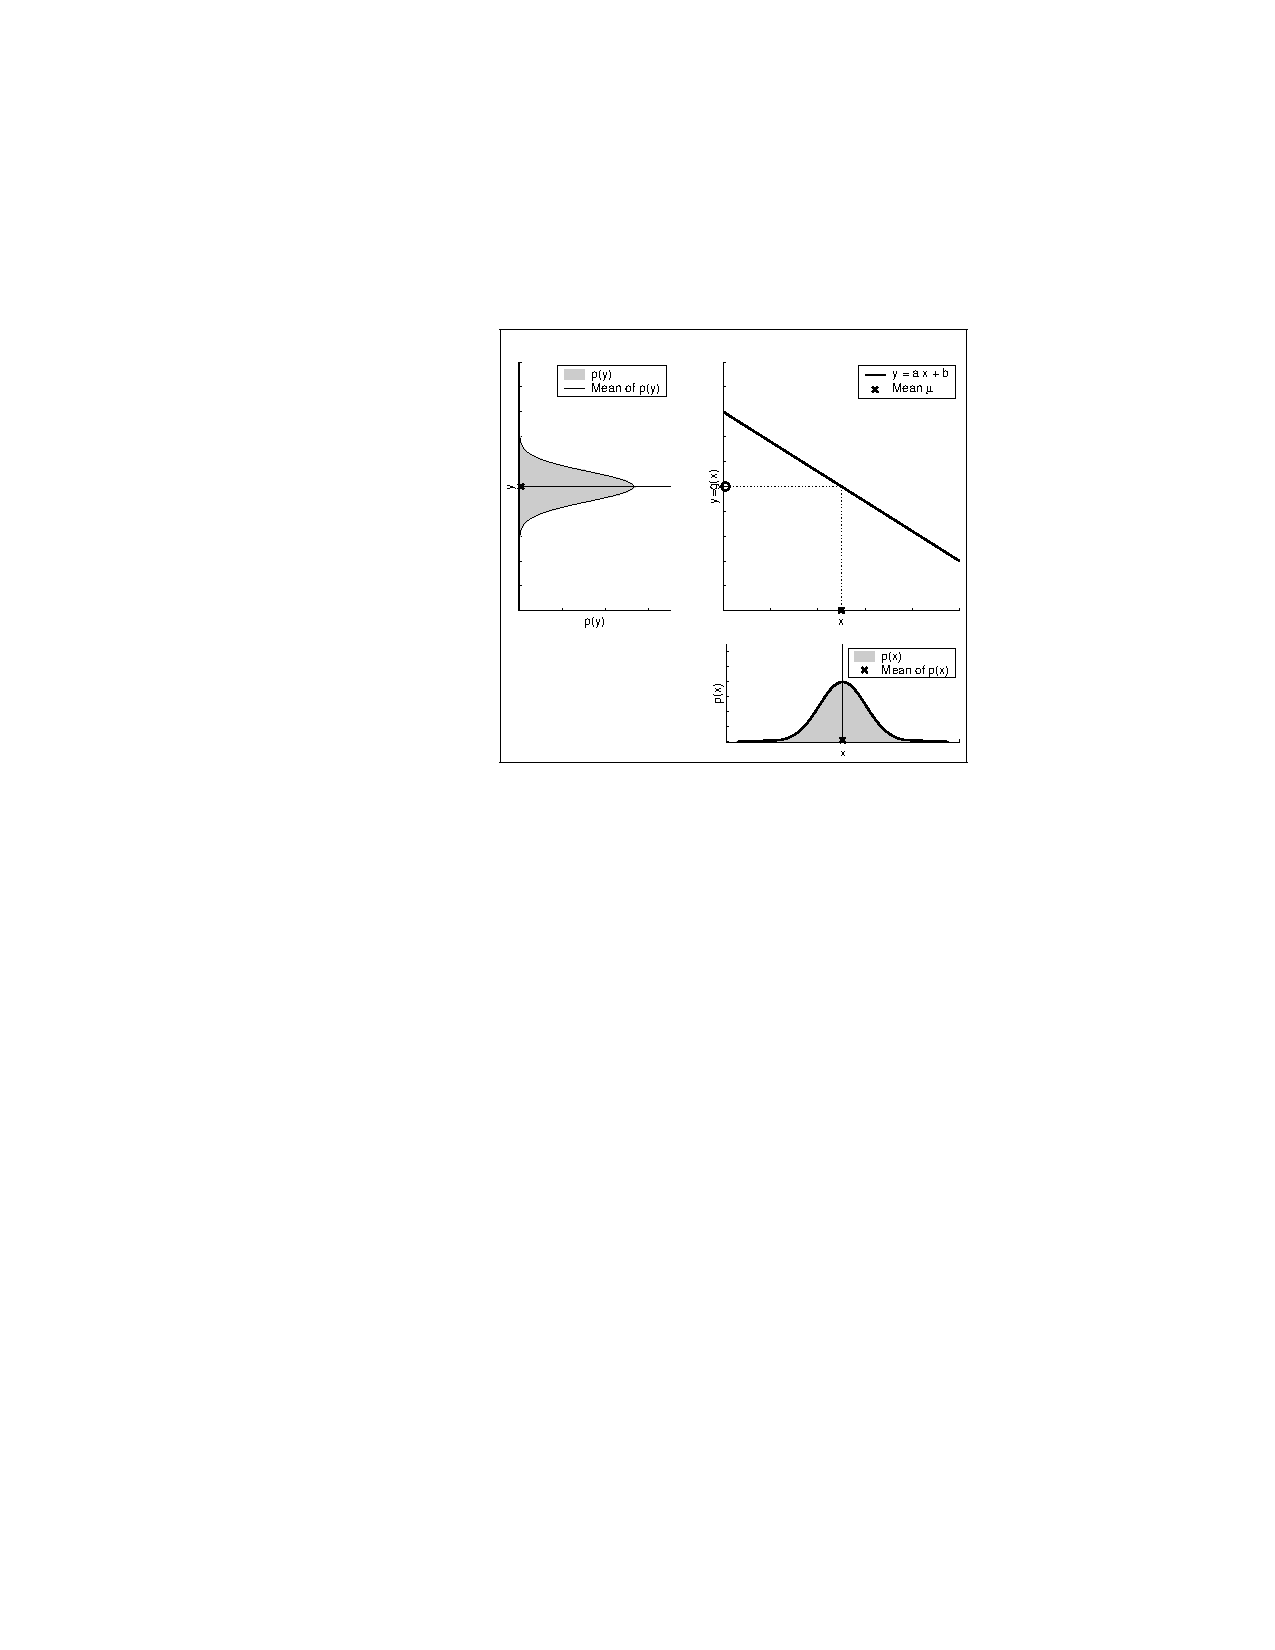
\includegraphics[width=3.5in]{./figures/KalmanXform.pdf}
\caption{Linear transformation of a Gaussian random variable \cite{thrun}. The lower right plot show the density of the original random variable, X. This random variable is passed through the function displayed in the upper right graph (the transformation of the mean is indicated by the dotted line). The density of the resulting random variable Y is plotted in the upper left graph.}
\label{KalmanXform}
\end{figure}

For a Kalman filter to work, all the transformations need to be linear. Figure \ref{KalmanXform} illustrates the linear transform of a one-dimensional Gaussian random variable. The graph on the lower right shows the density of this random variable having mean $\mu$ and variance $\sigma^2$. The random variable is passed through a linear function $y=ax+b$ shown in the upper right graph. The resulting random variable will have Gaussian distribution with mean $a\mu + b$ and variance $a^2\sigma^2$. This resulting Gaussian is shown in the upper left graph of figure \ref{KalmanXform}.\\

Unfortunately state transitions and measurements are rarely linear in practice \cite{thrun}. This renders Kalman filters inapplicable to most robotics problems. The Extended Kalman filter, or EKF, relaxes one of the assumptions. Here the assumption is that state transition probabilities and landmark measurement probabilities are governed by nonlinear functions $g$ and $h$ respectively:
\begin{equation}\label{transition}
x_{t} = g(u_{t}, x_{t-1}) + \varepsilon_{t}
\end{equation}
\begin{equation}\label{measurement}
z_{t} = h(x_{t}) + \delta_{t}
\end{equation}

Here $x_{t}$ is the robot location at time $t$, $u_{t}$ is the robot command that causes it to reach position $x_{t}$, $z_{t}$ is the landmark measurement at time $t$, $\epsilon_{t}$ is the robot motion uncertainty that depends of the mechanical properties of the robot and $\delta_{t}$ is the sensor measurement uncertainty. \\

\begin{figure}[!t]
\centering
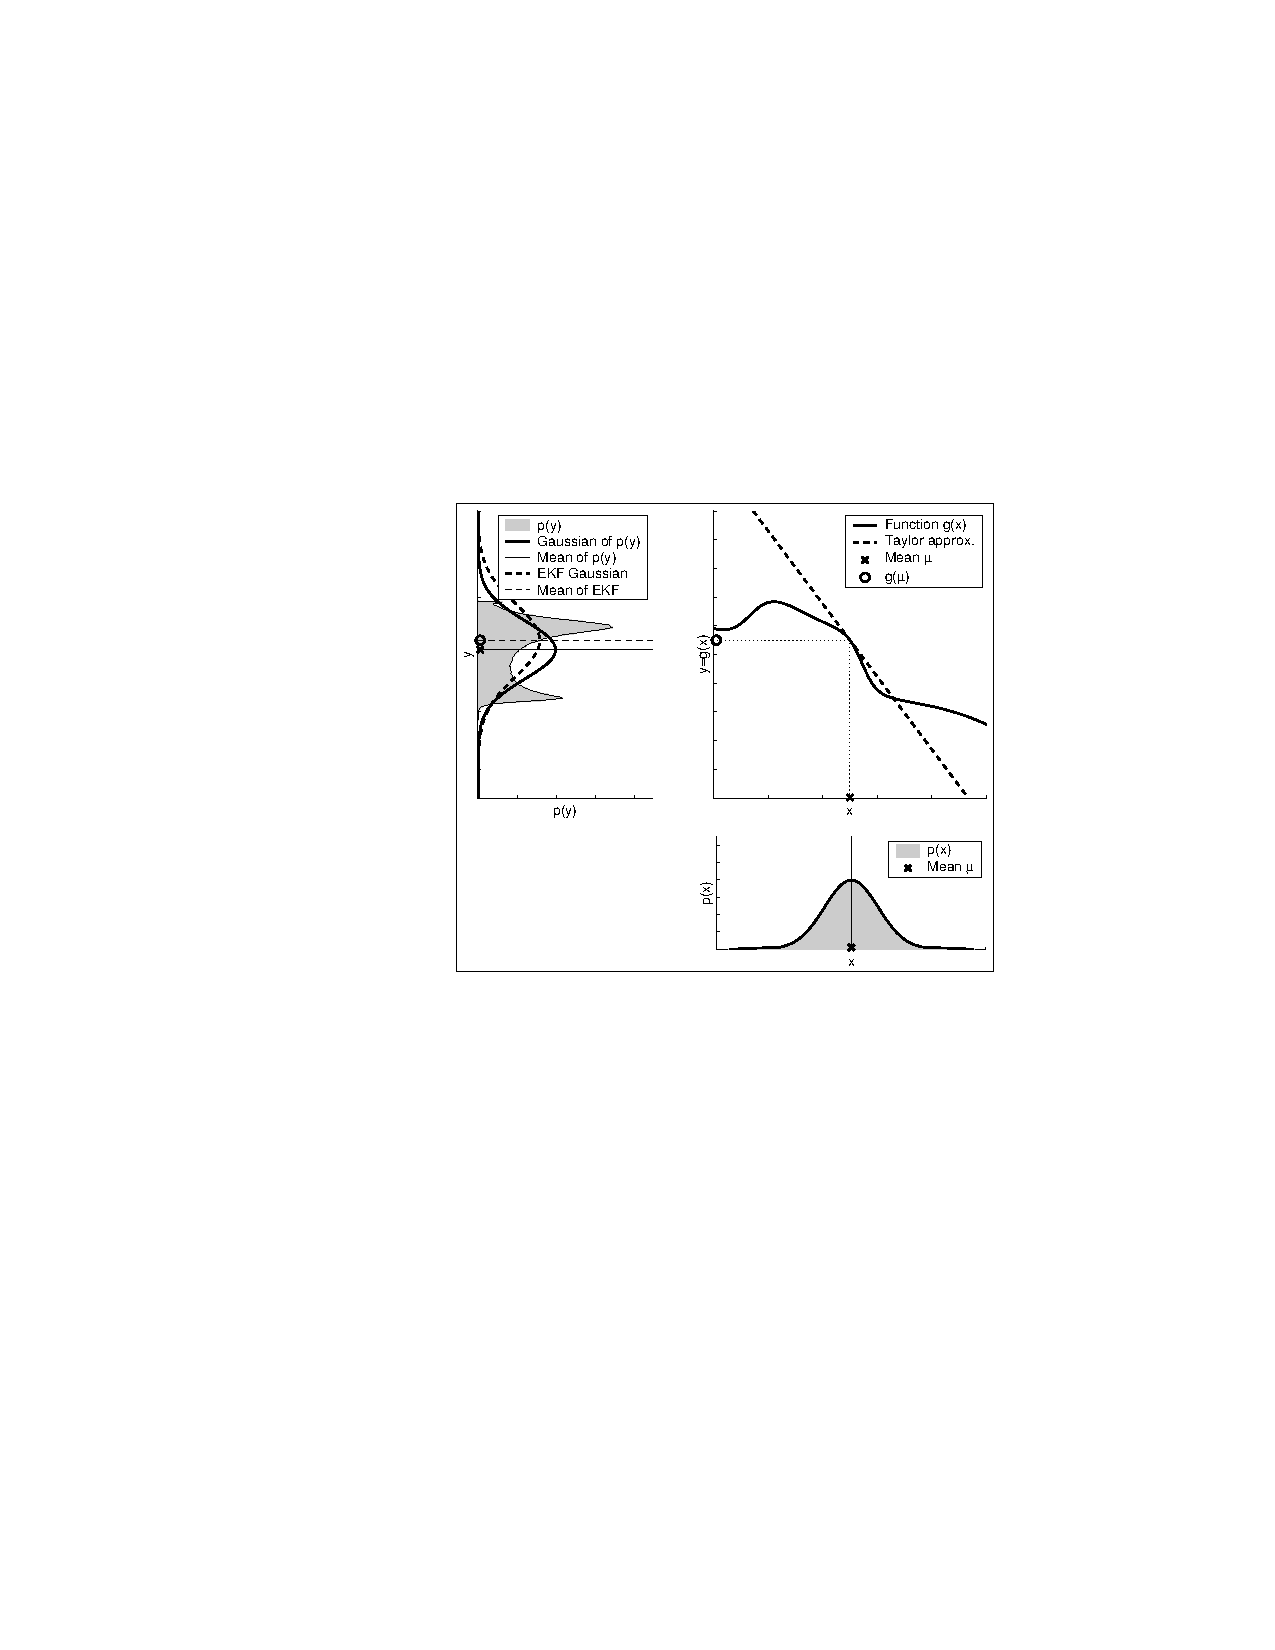
\includegraphics[width=3.5in]{./figures/EkfXform.pdf}
\caption{Illustration of linearization applied by the EKF \cite{thrun}. Instead of passing the Gaussian through the nonlinear function g, it is passed through a linear approximation of g. The linear function is tangent to g at the mean of the original Gaussian. The resulting Gaussian is shown as the dashed line in the upper left graph. The linearization incurs an approximation error, as indicated by the mismatch between the linearized Gaussian (dashed) and the Gaussian computed from the highly accurate Monte-Carlo estimate (solid).}
\label{EkfXform}
\end{figure}

Figure \ref{EkfXform} illustrates the impact of a nonlinear transformation on a Gaussian random variable. The graph on the upper right plots the nonlinear function $g$. As you can see, the transformed function is not a Gaussian. The idea behind the EKF is linearization. The nonlinear function is approximated at mean of the Gaussian. Projecting this Gaussian through this linear approximation results in a Gaussian density as represented by the dotted line in the upper left of figure \ref{EkfXform}.\\

The Extended Kalman filter algorithm is given below

\begin{minipage}{\linewidth}
  \begin{algorithm}[H]
    \caption{Extended Kalman Filter Algorithm}\label{AlgEkf}
    \begin{algorithmic}[1]
      \Procedure{Extended Kalman Filter Algorithm} {$\mu_{t-1},\Sigma_{t-1}, u_t,z_t$}
	\State $\overline \mu_t = g(u_t, \mu_{t-1})$
	\State $\overline \Sigma_t= G_t \Sigma_{t-1} G_t^T + R_t$  
	\State $K_t = \overline \Sigma_t H_t^T{(H_t \overline \Sigma_t H_t^T + Q_t)}^{-1}$
	\State $\mu_t = \overline \mu_t + K_t(z_t - h(\overline \mu_t))$
	\State $\Sigma_t = (I - K_t H_t) \overline \Sigma_t$
	\State return $\mu_t, \Sigma_t$
      \EndProcedure
    \end{algorithmic}
  \end{algorithm}
\end{minipage}\\\\

As can be seen, the EKF algorithm is similar to the Kalman filter algorithm in may ways. EKFs use Jacobians $G_t$ and $H_t$ instead of the corresponding linear system matrices $A_t$, $B_t$ and $C_t$ in Kalman filters. The Jacobian $G_t$ corresponds to the matrices $A_t$ and $B_t$, and the Jacobian $H_t$ corresponds to $C_t$. The Jacobians are actually the linear approximations of the non-linear functions at the mean of the random variable that is being transformed.
\subsection{Implementing the EKF}

Python libraries used and GoPiGo libraries
Calibration of the robot movement and sensing. Provide reference to data in section VII
Computing covariance matrices for movement and sensing
Movement using encoders. Forward, backwards and rotate in place.
Sense obstacles and return range and bearing
Obstacle Navigation using above functions
Movement equations
Robot pose prediction, movement jacobian and pose covariance
Problems in rangefinder accuracy
Correction step not implemented

\section{Results}
Sebsor accuracy problem
Robot residual drift handled by covariance
Sense inaccuracy covered by covariance

\section{Discussion}
The kalman gain and its awesome potential
Uses in rockets, missiles, battery charge estimation

\section{Conclusions and Future work}
Need better sensor. Investigate x-box sensor for range and visual


% An example of a floating figure using the graphicx package.
% Note that \label must occur AFTER (or within) \caption.
% For figures, \caption should occur after the \includegraphics.
% Note that IEEEtran v1.7 and later has special internal code that
% is designed to preserve the operation of \label within \caption
% even when the captionsoff option is in effect. However, because
% of issues like this, it may be the safest practice to put all your
% \label just after \caption rather than within \caption{}.
%
% Reminder: the "draftcls" or "draftclsnofoot", not "draft", class
% option should be used if it is desired that the figures are to be
% displayed while in draft mode.
%
%\begin{figure}[!t]
%\centering
%\includegraphics[width=2.5in]{myfigure}
% where an .eps filename suffix will be assumed under latex, 
% and a .pdf suffix will be assumed for pdflatex; or what has been declared
% via \DeclareGraphicsExtensions.
%\caption{Simulation results for the network.}
%\label{fig_sim}
%\end{figure}

% Note that the IEEE typically puts floats only at the top, even when this
% results in a large percentage of a column being occupied by floats.


% An example of a double column floating figure using two subfigures.
% (The subfig.sty package must be loaded for this to work.)
% The subfigure \label commands are set within each subfloat command,
% and the \label for the overall figure must come after \caption.
% \hfil is used as a separator to get equal spacing.
% Watch out that the combined width of all the subfigures on a 
% line do not exceed the text width or a line break will occur.
%
%\begin{figure*}[!t]
%\centering
%\subfloat[Case I]{\includegraphics[width=2.5in]{box}%
%\label{fig_first_case}}
%\hfil
%\subfloat[Case II]{\includegraphics[width=2.5in]{box}%
%\label{fig_second_case}}
%\caption{Simulation results for the network.}
%\label{fig_sim}
%\end{figure*}
%
% Note that often IEEE papers with subfigures do not employ subfigure
% captions (using the optional argument to \subfloat[]), but instead will
% reference/describe all of them (a), (b), etc., within the main caption.
% Be aware that for subfig.sty to generate the (a), (b), etc., subfigure
% labels, the optional argument to \subfloat must be present. If a
% subcaption is not desired, just leave its contents blank,
% e.g., \subfloat[].


% An example of a floating table. Note that, for IEEE style tables, the
% \caption command should come BEFORE the table and, given that table
% captions serve much like titles, are usually capitalized except for words
% such as a, an, and, as, at, but, by, for, in, nor, of, on, or, the, to
% and up, which are usually not capitalized unless they are the first or
% last word of the caption. Table text will default to \footnotesize as
% the IEEE normally uses this smaller font for tables.
% The \label must come after \caption as always.
%
%\begin{table}[!t]
%% increase table row spacing, adjust to taste
%\renewcommand{\arraystretch}{1.3}
% if using array.sty, it might be a good idea to tweak the value of
% \extrarowheight as needed to properly center the text within the cells
%\caption{An Example of a Table}
%\label{table_example}
%\centering
%% Some packages, such as MDW tools, offer better commands for making tables
%% than the plain LaTeX2e tabular which is used here.
%\begin{tabular}{|c||c|}
%\hline
%One & Two\\
%\hline
%Three & Four\\
%\hline
%\end{tabular}
%\end{table}


% Note that the IEEE does not put floats in the very first column
% - or typically anywhere on the first page for that matter. Also,
% in-text middle ("here") positioning is typically not used, but it
% is allowed and encouraged for Computer Society conferences (but
% not Computer Society journals). Most IEEE journals/conferences use
% top floats exclusively. 
% Note that, LaTeX2e, unlike IEEE journals/conferences, places
% footnotes above bottom floats. This can be corrected via the
% \fnbelowfloat command of the stfloats package.







% conference papers do not normally have an appendix


% use section* for acknowledgment






% trigger a \newpage just before the given reference
% number - used to balance the columns on the last page
% adjust value as needed - may need to be readjusted if
% the document is modified later
%\IEEEtriggeratref{8}
% The "triggered" command can be changed if desired:
%\IEEEtriggercmd{\enlargethispage{-5in}}

% references section

% can use a bibliography generated by BibTeX as a .bbl file
% BibTeX documentation can be easily obtained at:
% http://mirror.ctan.org/biblio/bibtex/contrib/doc/
% The IEEEtran BibTeX style support page is at:
% http://www.michaelshell.org/tex/ieeetran/bibtex/
%\bibliographystyle{IEEEtran}
% argument is your BibTeX string definitions and bibliography database(s)
%\bibliography{IEEEabrv,../bib/paper}
%
% <OR> manually copy in the resultant .bbl file
% set second argument of \begin to the number of references
% (used to reserve space for the reference number labels box)
\begin{thebibliography}{1}

\bibitem{dexter}
GoPiGo - Dexter Industries. \emph{Dexter Industries}. N.p., n.d. Web. 06 Nov. 2015. \url{http://www.dexterindustries.com/gopigo/}.

\bibitem{slam1}
Durrant-Whyte, H., and T. Bailey, \emph{Simultaneous Localization and Mapping: Part I}, IEEE Robotics and Automation Magazine. 13.2 (2006): 99-110.

\bibitem{slam2}
Bailey, Tim, and Hugh Durrant-Whyte, \emph{Simultaneous localization and mapping (SLAM): Part II}, IEEE Robotics and Automation Magazine. 13.3 (2006): 108-117.

\bibitem{thrun}
Thrun, Sebastian, Wolfram Burgard, and Dieter Fox, \emph{Probabilistic Robotics}, MIT press, 2005.

\bibitem{stachniss}
Stachniss, Cyrill, \emph{SLAM Course - WS13/14}, YouTube. YouTube, n.d. Web. 18 Sept. 2015. \url{https://www.youtube.com/ playlist?list=PLgnQpQtFTOGQrZ4O5QzbIHgl3b1JHimN_}.

\bibitem{maybeck}
Maybeck, Peter S., and George M. Siouris. "Stochastic models, estimation, and control, volume i." IEEE Transactions on Systems, Man, and Cybernetics 5.10 (1980): 282.

\end{thebibliography}

\section{Supplementary Materials}
\subsection{Combining two Gaussian distributions}
\label{sssec:num1} 
Figure \ref{CombineGaussians} shows two Gaussian distributions for the position of a robot in dotted lines with means $z_1$ and $z_2$ and standard deviations $\sigma_{z_1}$ and $\sigma_{z_2}$ respectively. The resulting distribution obtained by combining these two distributions is shown in the solid line with mean $\mu$ and standard deviation $\sigma$.\\

The mean for the resulting distribution is given by \cite{maybeck}
\begin{equation}\label{CombinedMean}
\mu = (\frac{\sigma_{z_2}^2}{\sigma_{z_1}^2 + \sigma_{z_2}^2})z_1 + (\frac{\sigma_{z_1}^2}{\sigma_{z_1}^2 + \sigma_{z_2}^2})z_2
\end{equation}

and the variance for the resulting distribution is given by

\begin{equation}\label{CombinedVariance}
\frac{1}{\sigma^2}=\frac{1}{\sigma_{z_1}^2}+\frac{1}{\sigma_{z_2}^2}
\end{equation}

\begin{figure}
\centering
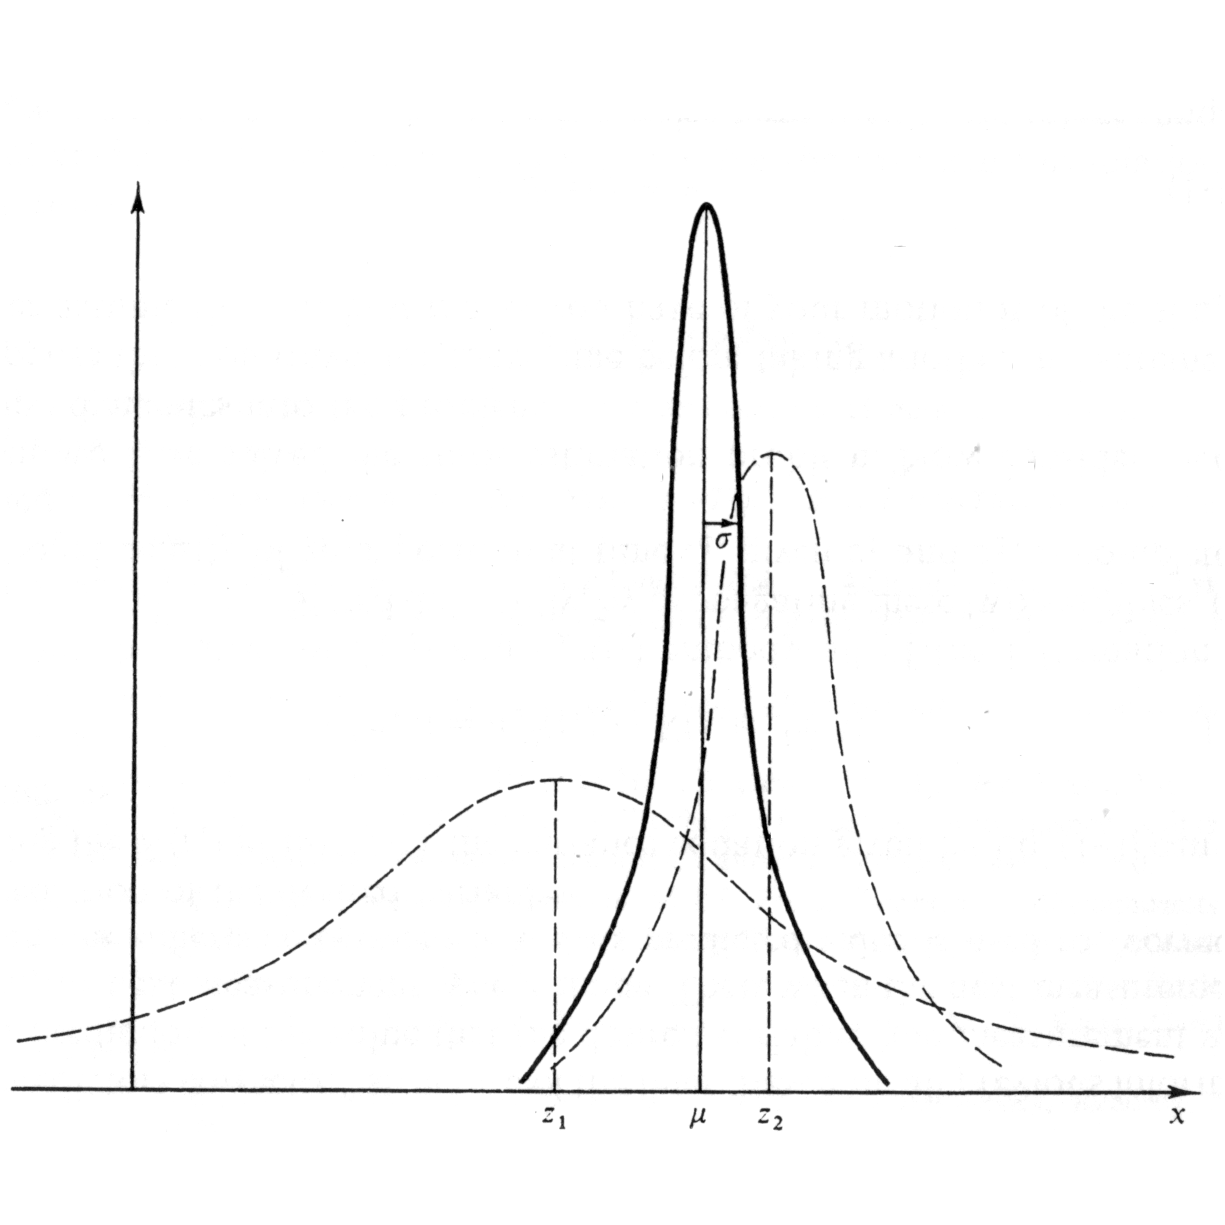
\includegraphics[width=3.5in, height=3.5in]{./figures/CombineGaussians.png}
\caption{Conditional density of position based on data $z_1$ and $z_2$ \cite{maybeck}. x-axis=position, y-axis-probability of being at the position}
\label{CombineGaussians}
\end{figure}

If the uncertainties $\sigma_{z_1}$ and $\sigma_{z_2}$ of the two distributions are equal, based on equation \ref{CombinedMean} the expected mean of the resulting distribution (the expected robot position) is just the average of the two or in other words, a position exactly between the two locations $\sigma_{z_1}$ and $\sigma_{z_2}$ \cite{maybeck}.\\

On the other hand if $\sigma_{z_1}$ were larger than $\sigma_{z_2}$, which is to say that the uncertainty involved in the measurement of $z_1$ is greater than that of $z_2$, then equation \ref{CombinedMean} dictates weighing $z_2$ more heavily than $z_1$. Which means the expected robot position will be closer to $z_2$. This is the scenario shown in figure \ref{CombineGaussians}.\\

As per equation \ref{CombinedVariance}, the uncertainty of the resulting distribution is less than $\sigma_{z_2}$ even if $\sigma_{z_1}$ is very large. That is to say that the uncertainty of the resulting distribution is less than either of the two uncertainties. This may seem counter-intuitive, but even if very poor quality data is taken into consideration, it does provide some information and thus will increase the precision of a measurement.

% that's all folks
\end{document}


